% Created by tikzDevice version 0.12.6 on 2026-05-06 11:22:51
% !TEX encoding = UTF-8 Unicode
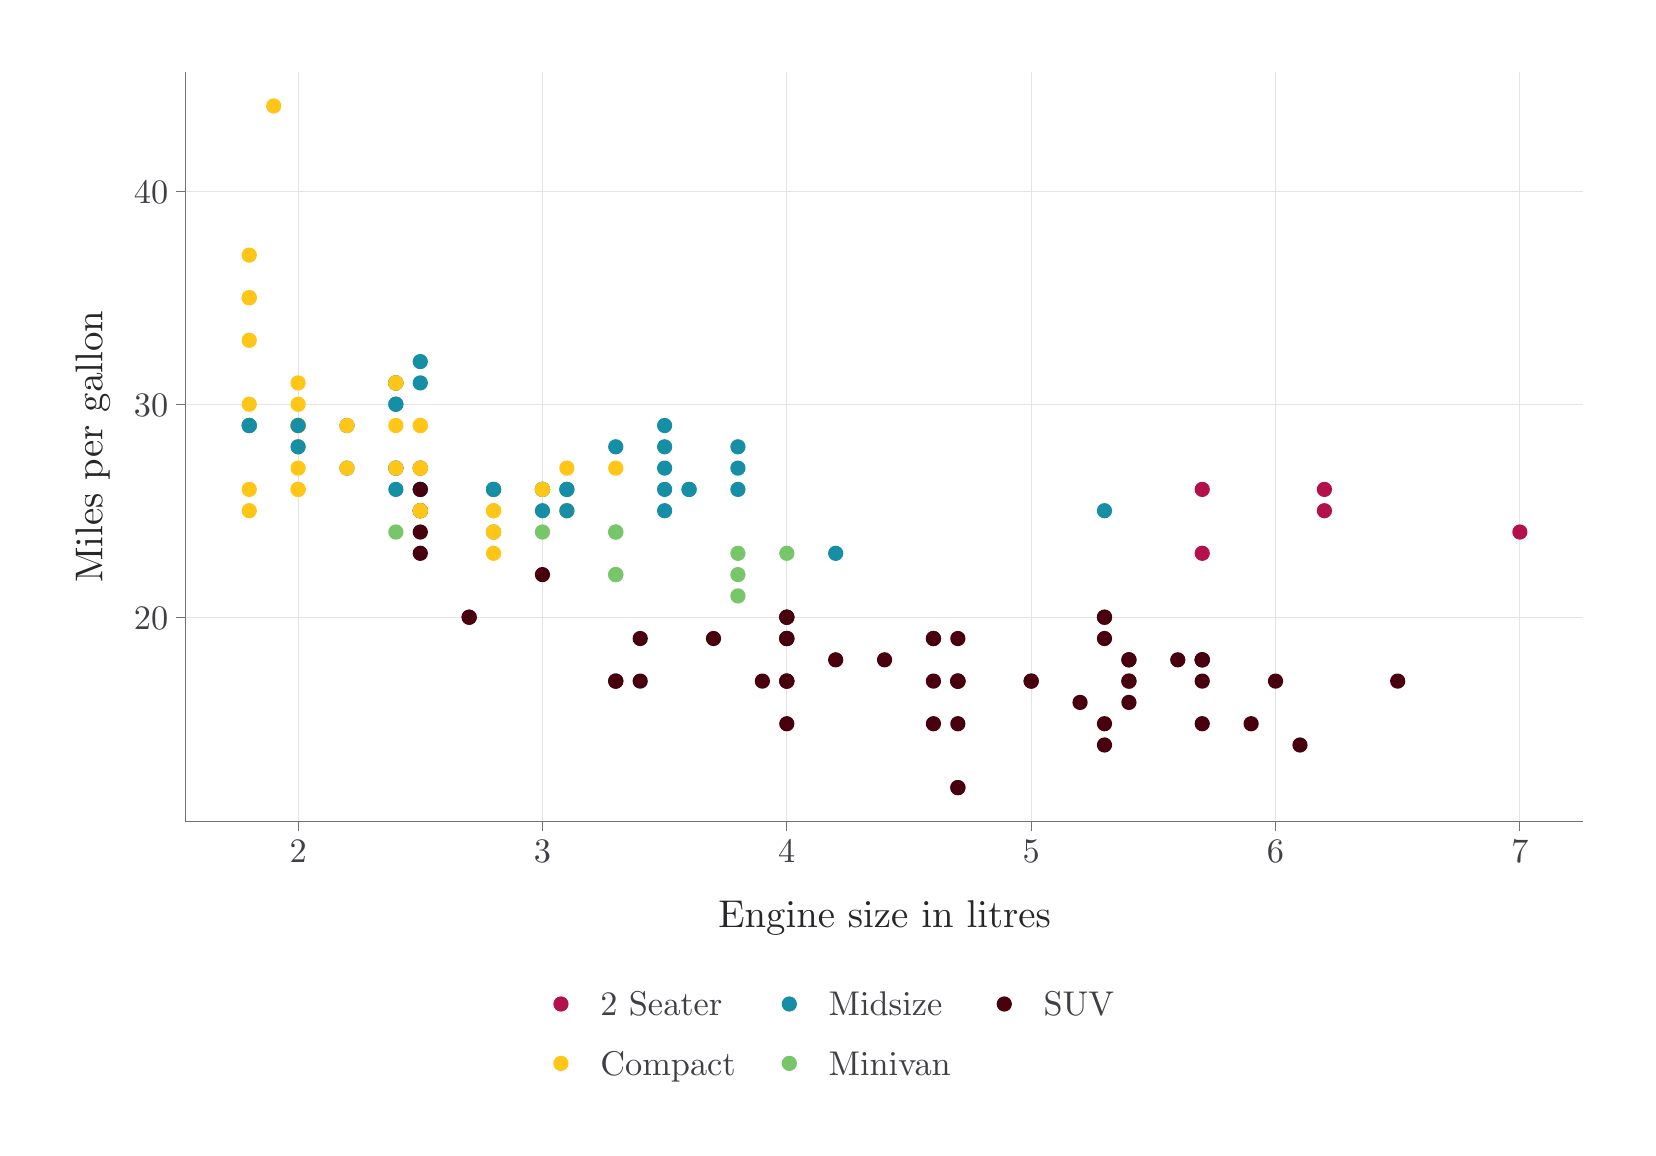
\begin{tikzpicture}[x=1pt,y=1pt]
\definecolor{fillColor}{RGB}{255,255,255}
\path[use as bounding box,fill=fillColor] (0,0) rectangle (578.16,397.48);
\begin{scope}
\path[clip] (  0.00,  0.00) rectangle (578.16,397.48);
\definecolor{drawColor}{RGB}{255,255,255}

\path[draw=drawColor,line width= 0.7pt,line join=round,line cap=round,fill=fillColor] (  0.00,  0.00) rectangle (578.16,397.48);
\end{scope}
\begin{scope}
\path[clip] ( 57.10,110.56) rectangle (562.16,381.48);
\definecolor{drawColor}{RGB}{255,255,255}
\definecolor{fillColor}{RGB}{255,255,255}

\path[draw=drawColor,line width= 0.7pt,line join=round,line cap=round,fill=fillColor] ( 57.10,110.56) rectangle (562.16,381.48);
\definecolor{drawColor}{RGB}{228,228,231}

\path[draw=drawColor,line width= 0.4pt,line join=round] ( 57.10,184.45) --
	(562.16,184.45);

\path[draw=drawColor,line width= 0.4pt,line join=round] ( 57.10,261.41) --
	(562.16,261.41);

\path[draw=drawColor,line width= 0.4pt,line join=round] ( 57.10,338.38) --
	(562.16,338.38);

\path[draw=drawColor,line width= 0.4pt,line join=round] ( 97.72,110.56) --
	( 97.72,381.48);

\path[draw=drawColor,line width= 0.4pt,line join=round] (186.01,110.56) --
	(186.01,381.48);

\path[draw=drawColor,line width= 0.4pt,line join=round] (274.31,110.56) --
	(274.31,381.48);

\path[draw=drawColor,line width= 0.4pt,line join=round] (362.61,110.56) --
	(362.61,381.48);

\path[draw=drawColor,line width= 0.4pt,line join=round] (450.91,110.56) --
	(450.91,381.48);

\path[draw=drawColor,line width= 0.4pt,line join=round] (539.20,110.56) --
	(539.20,381.48);
\definecolor{drawColor}{RGB}{255,197,23}
\definecolor{fillColor}{RGB}{255,197,23}

\path[draw=drawColor,line width= 0.5pt,line join=round,line cap=round,fill=fillColor] ( 80.06,253.72) circle (  2.50);

\path[draw=drawColor,line width= 0.5pt,line join=round,line cap=round,fill=fillColor] ( 80.06,253.72) circle (  2.50);

\path[draw=drawColor,line width= 0.5pt,line join=round,line cap=round,fill=fillColor] ( 97.72,269.11) circle (  2.50);

\path[draw=drawColor,line width= 0.5pt,line join=round,line cap=round,fill=fillColor] ( 97.72,261.41) circle (  2.50);

\path[draw=drawColor,line width= 0.5pt,line join=round,line cap=round,fill=fillColor] (168.35,230.63) circle (  2.50);

\path[draw=drawColor,line width= 0.5pt,line join=round,line cap=round,fill=fillColor] (168.35,230.63) circle (  2.50);

\path[draw=drawColor,line width= 0.5pt,line join=round,line cap=round,fill=fillColor] (194.84,238.32) circle (  2.50);

\path[draw=drawColor,line width= 0.5pt,line join=round,line cap=round,fill=fillColor] ( 80.06,230.63) circle (  2.50);

\path[draw=drawColor,line width= 0.5pt,line join=round,line cap=round,fill=fillColor] ( 80.06,222.93) circle (  2.50);

\path[draw=drawColor,line width= 0.5pt,line join=round,line cap=round,fill=fillColor] ( 97.72,246.02) circle (  2.50);

\path[draw=drawColor,line width= 0.5pt,line join=round,line cap=round,fill=fillColor] ( 97.72,238.32) circle (  2.50);

\path[draw=drawColor,line width= 0.5pt,line join=round,line cap=round,fill=fillColor] (168.35,222.93) circle (  2.50);

\path[draw=drawColor,line width= 0.5pt,line join=round,line cap=round,fill=fillColor] (168.35,222.93) circle (  2.50);

\path[draw=drawColor,line width= 0.5pt,line join=round,line cap=round,fill=fillColor] (194.84,222.93) circle (  2.50);

\path[draw=drawColor,line width= 0.5pt,line join=round,line cap=round,fill=fillColor] (194.84,222.93) circle (  2.50);
\definecolor{drawColor}{RGB}{21,142,166}
\definecolor{fillColor}{RGB}{21,142,166}

\path[draw=drawColor,line width= 0.5pt,line join=round,line cap=round,fill=fillColor] (168.35,215.23) circle (  2.50);

\path[draw=drawColor,line width= 0.5pt,line join=round,line cap=round,fill=fillColor] (194.84,222.93) circle (  2.50);

\path[draw=drawColor,line width= 0.5pt,line join=round,line cap=round,fill=fillColor] (291.97,207.54) circle (  2.50);
\definecolor{drawColor}{RGB}{72,0,15}
\definecolor{fillColor}{RGB}{72,0,15}

\path[draw=drawColor,line width= 0.5pt,line join=round,line cap=round,fill=fillColor] (389.10,184.45) circle (  2.50);

\path[draw=drawColor,line width= 0.5pt,line join=round,line cap=round,fill=fillColor] (389.10,145.96) circle (  2.50);

\path[draw=drawColor,line width= 0.5pt,line join=round,line cap=round,fill=fillColor] (389.10,184.45) circle (  2.50);

\path[draw=drawColor,line width= 0.5pt,line join=round,line cap=round,fill=fillColor] (424.42,161.36) circle (  2.50);

\path[draw=drawColor,line width= 0.5pt,line join=round,line cap=round,fill=fillColor] (450.91,161.36) circle (  2.50);
\definecolor{drawColor}{RGB}{179,17,75}
\definecolor{fillColor}{RGB}{179,17,75}

\path[draw=drawColor,line width= 0.5pt,line join=round,line cap=round,fill=fillColor] (424.42,230.63) circle (  2.50);

\path[draw=drawColor,line width= 0.5pt,line join=round,line cap=round,fill=fillColor] (424.42,207.54) circle (  2.50);

\path[draw=drawColor,line width= 0.5pt,line join=round,line cap=round,fill=fillColor] (468.57,230.63) circle (  2.50);

\path[draw=drawColor,line width= 0.5pt,line join=round,line cap=round,fill=fillColor] (468.57,222.93) circle (  2.50);

\path[draw=drawColor,line width= 0.5pt,line join=round,line cap=round,fill=fillColor] (539.20,215.23) circle (  2.50);
\definecolor{drawColor}{RGB}{72,0,15}
\definecolor{fillColor}{RGB}{72,0,15}

\path[draw=drawColor,line width= 0.5pt,line join=round,line cap=round,fill=fillColor] (389.10,176.75) circle (  2.50);

\path[draw=drawColor,line width= 0.5pt,line join=round,line cap=round,fill=fillColor] (389.10,138.27) circle (  2.50);

\path[draw=drawColor,line width= 0.5pt,line join=round,line cap=round,fill=fillColor] (424.42,145.96) circle (  2.50);

\path[draw=drawColor,line width= 0.5pt,line join=round,line cap=round,fill=fillColor] (495.05,161.36) circle (  2.50);
\definecolor{drawColor}{RGB}{21,142,166}
\definecolor{fillColor}{RGB}{21,142,166}

\path[draw=drawColor,line width= 0.5pt,line join=round,line cap=round,fill=fillColor] (133.04,238.32) circle (  2.50);

\path[draw=drawColor,line width= 0.5pt,line join=round,line cap=round,fill=fillColor] (133.04,261.41) circle (  2.50);

\path[draw=drawColor,line width= 0.5pt,line join=round,line cap=round,fill=fillColor] (194.84,230.63) circle (  2.50);

\path[draw=drawColor,line width= 0.5pt,line join=round,line cap=round,fill=fillColor] (230.16,253.72) circle (  2.50);

\path[draw=drawColor,line width= 0.5pt,line join=round,line cap=round,fill=fillColor] (238.99,230.63) circle (  2.50);
\definecolor{drawColor}{RGB}{119,198,105}
\definecolor{fillColor}{RGB}{119,198,105}

\path[draw=drawColor,line width= 0.5pt,line join=round,line cap=round,fill=fillColor] (133.04,215.23) circle (  2.50);

\path[draw=drawColor,line width= 0.5pt,line join=round,line cap=round,fill=fillColor] (186.01,215.23) circle (  2.50);

\path[draw=drawColor,line width= 0.5pt,line join=round,line cap=round,fill=fillColor] (212.50,199.84) circle (  2.50);

\path[draw=drawColor,line width= 0.5pt,line join=round,line cap=round,fill=fillColor] (212.50,199.84) circle (  2.50);

\path[draw=drawColor,line width= 0.5pt,line join=round,line cap=round,fill=fillColor] (212.50,215.23) circle (  2.50);

\path[draw=drawColor,line width= 0.5pt,line join=round,line cap=round,fill=fillColor] (212.50,215.23) circle (  2.50);

\path[draw=drawColor,line width= 0.5pt,line join=round,line cap=round,fill=fillColor] (212.50,161.36) circle (  2.50);

\path[draw=drawColor,line width= 0.5pt,line join=round,line cap=round,fill=fillColor] (256.65,199.84) circle (  2.50);

\path[draw=drawColor,line width= 0.5pt,line join=round,line cap=round,fill=fillColor] (256.65,192.14) circle (  2.50);

\path[draw=drawColor,line width= 0.5pt,line join=round,line cap=round,fill=fillColor] (256.65,207.54) circle (  2.50);

\path[draw=drawColor,line width= 0.5pt,line join=round,line cap=round,fill=fillColor] (274.31,207.54) circle (  2.50);
\definecolor{drawColor}{RGB}{72,0,15}
\definecolor{fillColor}{RGB}{72,0,15}

\path[draw=drawColor,line width= 0.5pt,line join=round,line cap=round,fill=fillColor] (265.48,161.36) circle (  2.50);

\path[draw=drawColor,line width= 0.5pt,line join=round,line cap=round,fill=fillColor] (336.12,161.36) circle (  2.50);

\path[draw=drawColor,line width= 0.5pt,line join=round,line cap=round,fill=fillColor] (336.12,122.87) circle (  2.50);

\path[draw=drawColor,line width= 0.5pt,line join=round,line cap=round,fill=fillColor] (336.12,161.36) circle (  2.50);

\path[draw=drawColor,line width= 0.5pt,line join=round,line cap=round,fill=fillColor] (380.27,153.66) circle (  2.50);

\path[draw=drawColor,line width= 0.5pt,line join=round,line cap=round,fill=fillColor] (424.42,169.05) circle (  2.50);

\path[draw=drawColor,line width= 0.5pt,line join=round,line cap=round,fill=fillColor] (442.08,145.96) circle (  2.50);

\path[draw=drawColor,line width= 0.5pt,line join=round,line cap=round,fill=fillColor] (327.29,161.36) circle (  2.50);

\path[draw=drawColor,line width= 0.5pt,line join=round,line cap=round,fill=fillColor] (397.93,161.36) circle (  2.50);

\path[draw=drawColor,line width= 0.5pt,line join=round,line cap=round,fill=fillColor] (397.93,169.05) circle (  2.50);

\path[draw=drawColor,line width= 0.5pt,line join=round,line cap=round,fill=fillColor] (274.31,161.36) circle (  2.50);

\path[draw=drawColor,line width= 0.5pt,line join=round,line cap=round,fill=fillColor] (274.31,176.75) circle (  2.50);

\path[draw=drawColor,line width= 0.5pt,line join=round,line cap=round,fill=fillColor] (274.31,161.36) circle (  2.50);

\path[draw=drawColor,line width= 0.5pt,line join=round,line cap=round,fill=fillColor] (274.31,176.75) circle (  2.50);

\path[draw=drawColor,line width= 0.5pt,line join=round,line cap=round,fill=fillColor] (327.29,176.75) circle (  2.50);

\path[draw=drawColor,line width= 0.5pt,line join=round,line cap=round,fill=fillColor] (362.61,161.36) circle (  2.50);
\definecolor{drawColor}{RGB}{21,142,166}
\definecolor{fillColor}{RGB}{21,142,166}

\path[draw=drawColor,line width= 0.5pt,line join=round,line cap=round,fill=fillColor] (133.04,230.63) circle (  2.50);

\path[draw=drawColor,line width= 0.5pt,line join=round,line cap=round,fill=fillColor] (133.04,238.32) circle (  2.50);

\path[draw=drawColor,line width= 0.5pt,line join=round,line cap=round,fill=fillColor] (133.04,261.41) circle (  2.50);

\path[draw=drawColor,line width= 0.5pt,line join=round,line cap=round,fill=fillColor] (133.04,269.11) circle (  2.50);

\path[draw=drawColor,line width= 0.5pt,line join=round,line cap=round,fill=fillColor] (141.87,230.63) circle (  2.50);

\path[draw=drawColor,line width= 0.5pt,line join=round,line cap=round,fill=fillColor] (141.87,230.63) circle (  2.50);

\path[draw=drawColor,line width= 0.5pt,line join=round,line cap=round,fill=fillColor] (212.50,246.02) circle (  2.50);
\definecolor{drawColor}{RGB}{72,0,15}
\definecolor{fillColor}{RGB}{72,0,15}

\path[draw=drawColor,line width= 0.5pt,line join=round,line cap=round,fill=fillColor] (186.01,199.84) circle (  2.50);

\path[draw=drawColor,line width= 0.5pt,line join=round,line cap=round,fill=fillColor] (247.82,176.75) circle (  2.50);

\path[draw=drawColor,line width= 0.5pt,line join=round,line cap=round,fill=fillColor] (274.31,184.45) circle (  2.50);

\path[draw=drawColor,line width= 0.5pt,line join=round,line cap=round,fill=fillColor] (336.12,161.36) circle (  2.50);

\path[draw=drawColor,line width= 0.5pt,line join=round,line cap=round,fill=fillColor] (336.12,122.87) circle (  2.50);

\path[draw=drawColor,line width= 0.5pt,line join=round,line cap=round,fill=fillColor] (336.12,176.75) circle (  2.50);

\path[draw=drawColor,line width= 0.5pt,line join=round,line cap=round,fill=fillColor] (424.42,169.05) circle (  2.50);

\path[draw=drawColor,line width= 0.5pt,line join=round,line cap=round,fill=fillColor] (459.74,138.27) circle (  2.50);

\path[draw=drawColor,line width= 0.5pt,line join=round,line cap=round,fill=fillColor] (274.31,145.96) circle (  2.50);

\path[draw=drawColor,line width= 0.5pt,line join=round,line cap=round,fill=fillColor] (291.97,169.05) circle (  2.50);

\path[draw=drawColor,line width= 0.5pt,line join=round,line cap=round,fill=fillColor] (309.63,169.05) circle (  2.50);

\path[draw=drawColor,line width= 0.5pt,line join=round,line cap=round,fill=fillColor] (327.29,145.96) circle (  2.50);

\path[draw=drawColor,line width= 0.5pt,line join=round,line cap=round,fill=fillColor] (397.93,161.36) circle (  2.50);

\path[draw=drawColor,line width= 0.5pt,line join=round,line cap=round,fill=fillColor] (397.93,153.66) circle (  2.50);

\path[draw=drawColor,line width= 0.5pt,line join=round,line cap=round,fill=fillColor] (397.93,169.05) circle (  2.50);

\path[draw=drawColor,line width= 0.5pt,line join=round,line cap=round,fill=fillColor] (274.31,161.36) circle (  2.50);

\path[draw=drawColor,line width= 0.5pt,line join=round,line cap=round,fill=fillColor] (274.31,176.75) circle (  2.50);

\path[draw=drawColor,line width= 0.5pt,line join=round,line cap=round,fill=fillColor] (327.29,176.75) circle (  2.50);

\path[draw=drawColor,line width= 0.5pt,line join=round,line cap=round,fill=fillColor] (362.61,161.36) circle (  2.50);
\definecolor{drawColor}{RGB}{255,197,23}
\definecolor{fillColor}{RGB}{255,197,23}

\path[draw=drawColor,line width= 0.5pt,line join=round,line cap=round,fill=fillColor] (133.04,253.72) circle (  2.50);

\path[draw=drawColor,line width= 0.5pt,line join=round,line cap=round,fill=fillColor] (133.04,238.32) circle (  2.50);
\definecolor{drawColor}{RGB}{21,142,166}
\definecolor{fillColor}{RGB}{21,142,166}

\path[draw=drawColor,line width= 0.5pt,line join=round,line cap=round,fill=fillColor] (141.87,269.11) circle (  2.50);

\path[draw=drawColor,line width= 0.5pt,line join=round,line cap=round,fill=fillColor] (141.87,276.81) circle (  2.50);

\path[draw=drawColor,line width= 0.5pt,line join=round,line cap=round,fill=fillColor] (230.16,238.32) circle (  2.50);

\path[draw=drawColor,line width= 0.5pt,line join=round,line cap=round,fill=fillColor] (230.16,230.63) circle (  2.50);

\path[draw=drawColor,line width= 0.5pt,line join=round,line cap=round,fill=fillColor] (186.01,230.63) circle (  2.50);

\path[draw=drawColor,line width= 0.5pt,line join=round,line cap=round,fill=fillColor] (186.01,222.93) circle (  2.50);

\path[draw=drawColor,line width= 0.5pt,line join=round,line cap=round,fill=fillColor] (230.16,222.93) circle (  2.50);
\definecolor{drawColor}{RGB}{72,0,15}
\definecolor{fillColor}{RGB}{72,0,15}

\path[draw=drawColor,line width= 0.5pt,line join=round,line cap=round,fill=fillColor] (212.50,161.36) circle (  2.50);

\path[draw=drawColor,line width= 0.5pt,line join=round,line cap=round,fill=fillColor] (212.50,161.36) circle (  2.50);

\path[draw=drawColor,line width= 0.5pt,line join=round,line cap=round,fill=fillColor] (274.31,184.45) circle (  2.50);

\path[draw=drawColor,line width= 0.5pt,line join=round,line cap=round,fill=fillColor] (415.59,169.05) circle (  2.50);
\definecolor{drawColor}{RGB}{21,142,166}
\definecolor{fillColor}{RGB}{21,142,166}

\path[draw=drawColor,line width= 0.5pt,line join=round,line cap=round,fill=fillColor] (194.84,230.63) circle (  2.50);

\path[draw=drawColor,line width= 0.5pt,line join=round,line cap=round,fill=fillColor] (256.65,230.63) circle (  2.50);

\path[draw=drawColor,line width= 0.5pt,line join=round,line cap=round,fill=fillColor] (256.65,238.32) circle (  2.50);

\path[draw=drawColor,line width= 0.5pt,line join=round,line cap=round,fill=fillColor] (256.65,246.02) circle (  2.50);

\path[draw=drawColor,line width= 0.5pt,line join=round,line cap=round,fill=fillColor] (389.10,222.93) circle (  2.50);
\definecolor{drawColor}{RGB}{72,0,15}
\definecolor{fillColor}{RGB}{72,0,15}

\path[draw=drawColor,line width= 0.5pt,line join=round,line cap=round,fill=fillColor] (141.87,222.93) circle (  2.50);

\path[draw=drawColor,line width= 0.5pt,line join=round,line cap=round,fill=fillColor] (141.87,215.23) circle (  2.50);

\path[draw=drawColor,line width= 0.5pt,line join=round,line cap=round,fill=fillColor] (141.87,238.32) circle (  2.50);

\path[draw=drawColor,line width= 0.5pt,line join=round,line cap=round,fill=fillColor] (141.87,222.93) circle (  2.50);

\path[draw=drawColor,line width= 0.5pt,line join=round,line cap=round,fill=fillColor] (141.87,230.63) circle (  2.50);

\path[draw=drawColor,line width= 0.5pt,line join=round,line cap=round,fill=fillColor] (141.87,207.54) circle (  2.50);
\definecolor{drawColor}{RGB}{255,197,23}
\definecolor{fillColor}{RGB}{255,197,23}

\path[draw=drawColor,line width= 0.5pt,line join=round,line cap=round,fill=fillColor] (141.87,222.93) circle (  2.50);

\path[draw=drawColor,line width= 0.5pt,line join=round,line cap=round,fill=fillColor] (141.87,238.32) circle (  2.50);

\path[draw=drawColor,line width= 0.5pt,line join=round,line cap=round,fill=fillColor] (141.87,222.93) circle (  2.50);

\path[draw=drawColor,line width= 0.5pt,line join=round,line cap=round,fill=fillColor] (141.87,238.32) circle (  2.50);
\definecolor{drawColor}{RGB}{72,0,15}
\definecolor{fillColor}{RGB}{72,0,15}

\path[draw=drawColor,line width= 0.5pt,line join=round,line cap=round,fill=fillColor] (159.53,184.45) circle (  2.50);

\path[draw=drawColor,line width= 0.5pt,line join=round,line cap=round,fill=fillColor] (159.53,184.45) circle (  2.50);

\path[draw=drawColor,line width= 0.5pt,line join=round,line cap=round,fill=fillColor] (221.33,176.75) circle (  2.50);

\path[draw=drawColor,line width= 0.5pt,line join=round,line cap=round,fill=fillColor] (221.33,161.36) circle (  2.50);

\path[draw=drawColor,line width= 0.5pt,line join=round,line cap=round,fill=fillColor] (274.31,184.45) circle (  2.50);

\path[draw=drawColor,line width= 0.5pt,line join=round,line cap=round,fill=fillColor] (336.12,161.36) circle (  2.50);
\definecolor{drawColor}{RGB}{21,142,166}
\definecolor{fillColor}{RGB}{21,142,166}

\path[draw=drawColor,line width= 0.5pt,line join=round,line cap=round,fill=fillColor] (115.38,253.72) circle (  2.50);

\path[draw=drawColor,line width= 0.5pt,line join=round,line cap=round,fill=fillColor] (115.38,238.32) circle (  2.50);

\path[draw=drawColor,line width= 0.5pt,line join=round,line cap=round,fill=fillColor] (133.04,269.11) circle (  2.50);

\path[draw=drawColor,line width= 0.5pt,line join=round,line cap=round,fill=fillColor] (133.04,269.11) circle (  2.50);

\path[draw=drawColor,line width= 0.5pt,line join=round,line cap=round,fill=fillColor] (186.01,230.63) circle (  2.50);

\path[draw=drawColor,line width= 0.5pt,line join=round,line cap=round,fill=fillColor] (186.01,230.63) circle (  2.50);

\path[draw=drawColor,line width= 0.5pt,line join=round,line cap=round,fill=fillColor] (230.16,246.02) circle (  2.50);
\definecolor{drawColor}{RGB}{255,197,23}
\definecolor{fillColor}{RGB}{255,197,23}

\path[draw=drawColor,line width= 0.5pt,line join=round,line cap=round,fill=fillColor] (115.38,238.32) circle (  2.50);

\path[draw=drawColor,line width= 0.5pt,line join=round,line cap=round,fill=fillColor] (115.38,253.72) circle (  2.50);

\path[draw=drawColor,line width= 0.5pt,line join=round,line cap=round,fill=fillColor] (133.04,269.11) circle (  2.50);

\path[draw=drawColor,line width= 0.5pt,line join=round,line cap=round,fill=fillColor] (133.04,269.11) circle (  2.50);

\path[draw=drawColor,line width= 0.5pt,line join=round,line cap=round,fill=fillColor] (186.01,230.63) circle (  2.50);

\path[draw=drawColor,line width= 0.5pt,line join=round,line cap=round,fill=fillColor] (186.01,230.63) circle (  2.50);

\path[draw=drawColor,line width= 0.5pt,line join=round,line cap=round,fill=fillColor] (212.50,238.32) circle (  2.50);

\path[draw=drawColor,line width= 0.5pt,line join=round,line cap=round,fill=fillColor] ( 80.06,261.41) circle (  2.50);

\path[draw=drawColor,line width= 0.5pt,line join=round,line cap=round,fill=fillColor] ( 80.06,284.51) circle (  2.50);

\path[draw=drawColor,line width= 0.5pt,line join=round,line cap=round,fill=fillColor] ( 80.06,299.90) circle (  2.50);

\path[draw=drawColor,line width= 0.5pt,line join=round,line cap=round,fill=fillColor] ( 80.06,315.29) circle (  2.50);

\path[draw=drawColor,line width= 0.5pt,line join=round,line cap=round,fill=fillColor] ( 80.06,299.90) circle (  2.50);
\definecolor{drawColor}{RGB}{72,0,15}
\definecolor{fillColor}{RGB}{72,0,15}

\path[draw=drawColor,line width= 0.5pt,line join=round,line cap=round,fill=fillColor] (336.12,145.96) circle (  2.50);

\path[draw=drawColor,line width= 0.5pt,line join=round,line cap=round,fill=fillColor] (424.42,169.05) circle (  2.50);
\definecolor{drawColor}{RGB}{255,197,23}
\definecolor{fillColor}{RGB}{255,197,23}

\path[draw=drawColor,line width= 0.5pt,line join=round,line cap=round,fill=fillColor] ( 97.72,253.72) circle (  2.50);

\path[draw=drawColor,line width= 0.5pt,line join=round,line cap=round,fill=fillColor] ( 97.72,230.63) circle (  2.50);

\path[draw=drawColor,line width= 0.5pt,line join=round,line cap=round,fill=fillColor] ( 97.72,253.72) circle (  2.50);

\path[draw=drawColor,line width= 0.5pt,line join=round,line cap=round,fill=fillColor] ( 97.72,253.72) circle (  2.50);

\path[draw=drawColor,line width= 0.5pt,line join=round,line cap=round,fill=fillColor] (168.35,215.23) circle (  2.50);

\path[draw=drawColor,line width= 0.5pt,line join=round,line cap=round,fill=fillColor] ( 88.89,369.17) circle (  2.50);

\path[draw=drawColor,line width= 0.5pt,line join=round,line cap=round,fill=fillColor] ( 97.72,253.72) circle (  2.50);

\path[draw=drawColor,line width= 0.5pt,line join=round,line cap=round,fill=fillColor] ( 97.72,230.63) circle (  2.50);

\path[draw=drawColor,line width= 0.5pt,line join=round,line cap=round,fill=fillColor] ( 97.72,253.72) circle (  2.50);

\path[draw=drawColor,line width= 0.5pt,line join=round,line cap=round,fill=fillColor] ( 97.72,253.72) circle (  2.50);

\path[draw=drawColor,line width= 0.5pt,line join=round,line cap=round,fill=fillColor] (141.87,253.72) circle (  2.50);

\path[draw=drawColor,line width= 0.5pt,line join=round,line cap=round,fill=fillColor] (141.87,253.72) circle (  2.50);

\path[draw=drawColor,line width= 0.5pt,line join=round,line cap=round,fill=fillColor] (168.35,207.54) circle (  2.50);

\path[draw=drawColor,line width= 0.5pt,line join=round,line cap=round,fill=fillColor] (168.35,215.23) circle (  2.50);
\definecolor{drawColor}{RGB}{21,142,166}
\definecolor{fillColor}{RGB}{21,142,166}

\path[draw=drawColor,line width= 0.5pt,line join=round,line cap=round,fill=fillColor] ( 80.06,253.72) circle (  2.50);

\path[draw=drawColor,line width= 0.5pt,line join=round,line cap=round,fill=fillColor] ( 80.06,253.72) circle (  2.50);

\path[draw=drawColor,line width= 0.5pt,line join=round,line cap=round,fill=fillColor] ( 97.72,246.02) circle (  2.50);

\path[draw=drawColor,line width= 0.5pt,line join=round,line cap=round,fill=fillColor] ( 97.72,253.72) circle (  2.50);

\path[draw=drawColor,line width= 0.5pt,line join=round,line cap=round,fill=fillColor] (168.35,230.63) circle (  2.50);

\path[draw=drawColor,line width= 0.5pt,line join=round,line cap=round,fill=fillColor] (168.35,230.63) circle (  2.50);

\path[draw=drawColor,line width= 0.5pt,line join=round,line cap=round,fill=fillColor] (238.99,230.63) circle (  2.50);
\end{scope}
\begin{scope}
\path[clip] (  0.00,  0.00) rectangle (578.16,397.48);
\definecolor{drawColor}{RGB}{113,113,122}

\path[draw=drawColor,line width= 0.3pt,line join=round] ( 57.10,110.56) --
	( 57.10,381.48);
\end{scope}
\begin{scope}
\path[clip] (  0.00,  0.00) rectangle (578.16,397.48);
\definecolor{drawColor}{RGB}{63,63,70}

\node[text=drawColor,anchor=base east,inner sep=0pt, outer sep=0pt, scale=  1.24] at ( 50.80,180.16) {20};

\node[text=drawColor,anchor=base east,inner sep=0pt, outer sep=0pt, scale=  1.24] at ( 50.80,257.13) {30};

\node[text=drawColor,anchor=base east,inner sep=0pt, outer sep=0pt, scale=  1.24] at ( 50.80,334.10) {40};
\end{scope}
\begin{scope}
\path[clip] (  0.00,  0.00) rectangle (578.16,397.48);
\definecolor{drawColor}{RGB}{113,113,122}

\path[draw=drawColor,line width= 0.3pt,line join=round] ( 53.60,184.45) --
	( 57.10,184.45);

\path[draw=drawColor,line width= 0.3pt,line join=round] ( 53.60,261.41) --
	( 57.10,261.41);

\path[draw=drawColor,line width= 0.3pt,line join=round] ( 53.60,338.38) --
	( 57.10,338.38);
\end{scope}
\begin{scope}
\path[clip] (  0.00,  0.00) rectangle (578.16,397.48);
\definecolor{drawColor}{RGB}{113,113,122}

\path[draw=drawColor,line width= 0.3pt,line join=round] ( 57.10,110.56) --
	(562.16,110.56);
\end{scope}
\begin{scope}
\path[clip] (  0.00,  0.00) rectangle (578.16,397.48);
\definecolor{drawColor}{RGB}{113,113,122}

\path[draw=drawColor,line width= 0.3pt,line join=round] ( 97.72,107.06) --
	( 97.72,110.56);

\path[draw=drawColor,line width= 0.3pt,line join=round] (186.01,107.06) --
	(186.01,110.56);

\path[draw=drawColor,line width= 0.3pt,line join=round] (274.31,107.06) --
	(274.31,110.56);

\path[draw=drawColor,line width= 0.3pt,line join=round] (362.61,107.06) --
	(362.61,110.56);

\path[draw=drawColor,line width= 0.3pt,line join=round] (450.91,107.06) --
	(450.91,110.56);

\path[draw=drawColor,line width= 0.3pt,line join=round] (539.20,107.06) --
	(539.20,110.56);
\end{scope}
\begin{scope}
\path[clip] (  0.00,  0.00) rectangle (578.16,397.48);
\definecolor{drawColor}{RGB}{63,63,70}

\node[text=drawColor,anchor=base,inner sep=0pt, outer sep=0pt, scale=  1.24] at ( 97.72, 95.69) {2};

\node[text=drawColor,anchor=base,inner sep=0pt, outer sep=0pt, scale=  1.24] at (186.01, 95.69) {3};

\node[text=drawColor,anchor=base,inner sep=0pt, outer sep=0pt, scale=  1.24] at (274.31, 95.69) {4};

\node[text=drawColor,anchor=base,inner sep=0pt, outer sep=0pt, scale=  1.24] at (362.61, 95.69) {5};

\node[text=drawColor,anchor=base,inner sep=0pt, outer sep=0pt, scale=  1.24] at (450.91, 95.69) {6};

\node[text=drawColor,anchor=base,inner sep=0pt, outer sep=0pt, scale=  1.24] at (539.20, 95.69) {7};
\end{scope}
\begin{scope}
\path[clip] (  0.00,  0.00) rectangle (578.16,397.48);
\definecolor{drawColor}{RGB}{39,39,42}

\node[text=drawColor,anchor=base,inner sep=0pt, outer sep=0pt, scale=  1.40] at (309.63, 72.27) {Engine size in litres};
\end{scope}
\begin{scope}
\path[clip] (  0.00,  0.00) rectangle (578.16,397.48);
\definecolor{drawColor}{RGB}{39,39,42}

\node[text=drawColor,rotate= 90.00,anchor=base,inner sep=0pt, outer sep=0pt, scale=  1.40] at ( 27.00,246.02) {Miles per gallon};
\end{scope}
\begin{scope}
\path[clip] (  0.00,  0.00) rectangle (578.16,397.48);
\definecolor{drawColor}{RGB}{255,255,255}
\definecolor{fillColor}{RGB}{255,255,255}

\path[draw=drawColor,line width= 0.7pt,line join=round,line cap=round,fill=fillColor] (185.48, 16.00) rectangle (392.68, 56.91);
\end{scope}
\begin{scope}
\path[clip] (  0.00,  0.00) rectangle (578.16,397.48);
\definecolor{drawColor}{RGB}{255,255,255}
\definecolor{fillColor}{RGB}{255,255,255}

\path[draw=drawColor,line width= 0.7pt,line join=round,line cap=round,fill=fillColor] (185.48, 37.45) rectangle (199.93, 51.91);
\definecolor{drawColor}{RGB}{179,17,75}
\definecolor{fillColor}{RGB}{179,17,75}

\path[draw=drawColor,line width= 0.5pt,line join=round,line cap=round,fill=fillColor] (192.70, 44.68) circle (  2.50);
\end{scope}
\begin{scope}
\path[clip] (  0.00,  0.00) rectangle (578.16,397.48);
\definecolor{drawColor}{RGB}{255,255,255}
\definecolor{fillColor}{RGB}{255,255,255}

\path[draw=drawColor,line width= 0.7pt,line join=round,line cap=round,fill=fillColor] (185.48, 16.00) rectangle (199.93, 30.45);
\definecolor{drawColor}{RGB}{255,197,23}
\definecolor{fillColor}{RGB}{255,197,23}

\path[draw=drawColor,line width= 0.5pt,line join=round,line cap=round,fill=fillColor] (192.70, 23.23) circle (  2.50);
\end{scope}
\begin{scope}
\path[clip] (  0.00,  0.00) rectangle (578.16,397.48);
\definecolor{drawColor}{RGB}{255,255,255}
\definecolor{fillColor}{RGB}{255,255,255}

\path[draw=drawColor,line width= 0.7pt,line join=round,line cap=round,fill=fillColor] (267.99, 37.45) rectangle (282.44, 51.91);
\definecolor{drawColor}{RGB}{21,142,166}
\definecolor{fillColor}{RGB}{21,142,166}

\path[draw=drawColor,line width= 0.5pt,line join=round,line cap=round,fill=fillColor] (275.22, 44.68) circle (  2.50);
\end{scope}
\begin{scope}
\path[clip] (  0.00,  0.00) rectangle (578.16,397.48);
\definecolor{drawColor}{RGB}{255,255,255}
\definecolor{fillColor}{RGB}{255,255,255}

\path[draw=drawColor,line width= 0.7pt,line join=round,line cap=round,fill=fillColor] (267.99, 16.00) rectangle (282.44, 30.45);
\definecolor{drawColor}{RGB}{119,198,105}
\definecolor{fillColor}{RGB}{119,198,105}

\path[draw=drawColor,line width= 0.5pt,line join=round,line cap=round,fill=fillColor] (275.22, 23.23) circle (  2.50);
\end{scope}
\begin{scope}
\path[clip] (  0.00,  0.00) rectangle (578.16,397.48);
\definecolor{drawColor}{RGB}{255,255,255}
\definecolor{fillColor}{RGB}{255,255,255}

\path[draw=drawColor,line width= 0.7pt,line join=round,line cap=round,fill=fillColor] (345.66, 37.45) rectangle (360.12, 51.91);
\definecolor{drawColor}{RGB}{72,0,15}
\definecolor{fillColor}{RGB}{72,0,15}

\path[draw=drawColor,line width= 0.5pt,line join=round,line cap=round,fill=fillColor] (352.89, 44.68) circle (  2.50);
\end{scope}
\begin{scope}
\path[clip] (  0.00,  0.00) rectangle (578.16,397.48);
\definecolor{drawColor}{RGB}{63,63,70}

\node[text=drawColor,anchor=base west,inner sep=0pt, outer sep=0pt, scale=  1.24] at (206.93, 40.40) {2 Seater};
\end{scope}
\begin{scope}
\path[clip] (  0.00,  0.00) rectangle (578.16,397.48);
\definecolor{drawColor}{RGB}{63,63,70}

\node[text=drawColor,anchor=base west,inner sep=0pt, outer sep=0pt, scale=  1.24] at (206.93, 18.94) {Compact};
\end{scope}
\begin{scope}
\path[clip] (  0.00,  0.00) rectangle (578.16,397.48);
\definecolor{drawColor}{RGB}{63,63,70}

\node[text=drawColor,anchor=base west,inner sep=0pt, outer sep=0pt, scale=  1.24] at (289.44, 40.40) {Midsize};
\end{scope}
\begin{scope}
\path[clip] (  0.00,  0.00) rectangle (578.16,397.48);
\definecolor{drawColor}{RGB}{63,63,70}

\node[text=drawColor,anchor=base west,inner sep=0pt, outer sep=0pt, scale=  1.24] at (289.44, 18.94) {Minivan};
\end{scope}
\begin{scope}
\path[clip] (  0.00,  0.00) rectangle (578.16,397.48);
\definecolor{drawColor}{RGB}{63,63,70}

\node[text=drawColor,anchor=base west,inner sep=0pt, outer sep=0pt, scale=  1.24] at (367.12, 40.40) {SUV};
\end{scope}
\end{tikzpicture}
